\subsection*{The Thurston-Winkelnkemper construction}
\begin{definition}[mapping torus]
    Let $\Sigma$ be a smooth manifold with boundary $\partial \Sigma$ and $\phi: \Sigma \to \Sigma$ a diffeomorphism that is equal to the identity close to $\partial \Sigma$.
    The mapping torus $\Sigma(\phi)$ is given by
     $\Sigma \times [0,2\pi]/\sim$ where
     \[
        (x, 2\pi) \sim (\phi(x), 0). 
     \]
     The generalized mapping torus requires as additional data a smooth function $\overline{\varphi}: \Sigma \to \mathbb R^+$ that is constant near $\partial \Sigma$. Then,
     \[
        \Sigma_{\overline{\varphi}}(\phi) \coloneqq \Sigma \times \mathbb R/\sim \quad \text{where} \quad  (x, \theta) \sim (\phi(x), \theta - \overline{\varphi}(x)).
     \]
\end{definition}

\paragraph*{Abstract open books}
Starting with a mapping torus $\Sigma(\phi)$, we can construct an abstract open book $M(\phi)$ with binding $\partial \Sigma$ (see \cref{fig:abstract_open_book})
\begin{figure}[ht]
    \includegraphics*[width=\textwidth]{images/abstract_open_book.png}
    \caption[abstract open book]{highly professional drawing of an abstract open book}
    \label{fig:abstract_open_book}
\end{figure}

We define
\[
    M(\phi) \coloneqq \left(\Sigma(\phi) \cup \partial \Sigma \times D^2\right)/\sim
\]
where we identify
\[
    [x \in \partial \Sigma, \theta] \sim (x, r=1, \varphi = \theta)  
\]


\paragraph*{The construction}
Roadmap: 
\begin{itemize}
    \item Let 1-form on $\Sigma$ descend to mapping torus and add $+ \d \varphi$
    \item Extend this 1-form over the binding neighborhood of the open book
    \item Check that this actually gives a contact form with the desired properties
\end{itemize}

\paragraph*{Creating a contact form $\alpha$ on the mapping torus}
Let $\Sigma^{2n}$ be a compact manifold admitting an exact symplectic form $\omega = \d \beta$ s.t. on the boundary $\partial \Sigma$, a contact form $\beta_\partial$ is induced (this follows from the conditions requested in Geiges).
Let the boundary be connected (i.e. the binding is also connected).
Let the monodromy map $\phi$ be an exact symplectomorphism of $(\Sigma, \omega)$,
equal to the identity near the boundary $\partial \Sigma$ (exactness is not necessary according to Geiges, as it can be obtained via a suitable isotopy of the symplectomorphism).
An exact symplectomorphism $\phi$ of $(\Sigma, \omega)$ is such that
\[
    \phi^*(\beta) - \beta \eqqcolon \d \overline{\varphi}  
\]
is exact, i.e. there exists such a function $\overline{\varphi}$ on $\Sigma$ (of course only defined up to adding a locally constant function. Choose it in such a way that it only takes positive values).
The 1-form 
\[
    \alpha \coloneqq \beta + \d \varphi
\]
is a contact form on $\Sigma \times \mathbb R$:
\[
    \alpha \wedge (\d \alpha)^{n} = (\beta + \d \varphi)\wedge \underbrace{(\d \beta)^n}_{\eqqcolon \Omega} = \beta \wedge \Omega + \d \varphi \wedge \Omega = \d \varphi \wedge \Omega,
\]
where $\Omega$ is a volume form on $\Sigma$ (as $\beta$ is a symplectic form).
The $\beta \wedge \Omega$ term vanishes because both are forms on $\Sigma$, but $\Omega$ is already a top-level form.
The resulting form is a wedge product of two volume forms on the product manifolds and therefore a volume form on $\Sigma \times \mathbb R$.

Now consider the transformation that induces the generalized mapping torus
\[
    F \coloneqq (x,\varphi) \mapsto (\phi(x), \varphi - \overline{\varphi}(x)).    
\]
Remember that $\varphi$ only takes positive values, i.e. the mapping torus is welldefined.
The 1-form $\alpha$ is invariant under this transformation:
\begin{align*}
    F^*(\alpha) &= F^*(\beta) + F^*(\d \varphi)&&|\;\beta\text{ is independent of }\varphi\\
    &= \phi^*(\beta) + \d F(\varphi)&&|\text{ definition of }\overline{\varphi}, F\\
    &= \beta + \d\overline{\varphi} + \d \varphi - \d \overline{\varphi}\\
    &= \alpha.
\end{align*}
It follows that $\alpha$ descends to a contact form on $\Sigma_{\overline{\varphi}}(\phi)$. 

\paragraph*{Extending $\alpha$ to the whole abstract open book}

First, we describe a gluing construction for the abstract open book.
Therefore, we construct a collar neighborhood on the generalized mapping torus s.t. on $[-1,0] \times \partial \Sigma$, the symplectic form is given by $\d \left(e^s\beta_\partial\right)$ where $s$ is the collar parameter, d.h. $\beta = e^s\beta_\partial$.
\underline{Why does such a neighborhood exist?}

Close to $\partial \Sigma$, $\phi$ is equal to the identity and therefore $\d \overline{\varphi}$ is locally constant (hence constant, as $\partial \Sigma$ is connected).
Parametrize the neighborhood so that $\overline{\varphi}$ is constant on $[-1,0]\times \partial \Sigma$.

Now, take a look at
\[
    \left(\Sigma_{\overline{\varphi}}(\phi)\; \dot\cup\; \left(\partial \Sigma \times D_2^2\right)\right)/\sim.
\]
\begin{figure}
    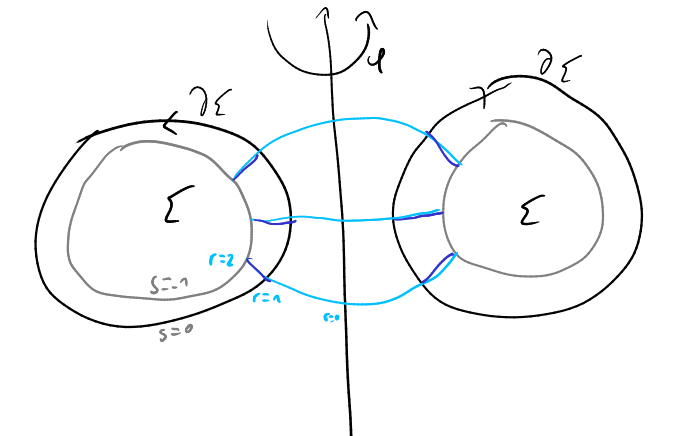
\includegraphics[width=\textwidth]{images/abstract_open_book_gluing.png}
    \caption[Glueing an abstract open book]{Detailled glueing process of the generalized abstract open book}
    \label{fig:abstract_open_book_gluing}
\end{figure}
A simple linear reparametrization will make the notation a lot easier: As $\overline{\varphi}$ is constant on the neighborhood under consideration, we just pretend $\overline{\varphi} = 2\pi$.
Furthermore, we parametrize the boundary $\partial \Sigma$ with $\theta \in S^1$.
Then we identify 
\[
    (s, \theta, \varphi) \in [-1,0] \times \partial \Sigma \times S^1 \subset \Sigma_{\overline{\varphi}}(\phi)
\]
with
\[
    (\theta, s = 1-r, \varphi) \in \partial \Sigma \times D_2^2
\]
where $(r, \varphi)$ are polar coordinates on $D_2^2$, i.e. we identify a collar neighborhood of $\Sigma$ with an annulus in $D_2^2$.
(See \cref{fig:abstract_open_book_gluing})


Now we choose the ansatz
\[
    \alpha_\text{ext} \coloneqq h_1(r) \beta_\partial + h_2(r) \d\varphi.
\]
for the extension of the contact form over $\partial \Sigma \times D^2$.
On the gluing area (i.e. $1 \le r \le 2$), $\alpha_\text{ext}$ has to agree with $\alpha = \beta + \d \varphi = e^s \beta_\partial + \d \varphi$,
d.h.
\[
    h_1(r) = e^s = e^{1-r} \qquad h_2(r) = 1.
\]
In order to ensure smoothness at $r=0$, in a small neighborhood of $r = 0$ we set $h_1(r) = 2$ and $h_2(r) = r^2$, obtaining
\[
    \alpha_\text{ext} = 2\beta_\partial + r^2\d \varphi.
\] 
We compute
\[
    \d \alpha_\text{ext} = h_1'(r)\d r\wedge \beta_\partial + h_1(r) \d \beta_\partial + h_2'(r) \d r \wedge \d\varphi.
\]
and
\[
    (\d \alpha_\text{ext})^n = n\cdot \d r\wedge (h_1'(r) \beta_\partial + h_2'(r) \d\varphi) \cdot h_1(r)^{n-1}(\d \beta_\partial)^{n-1} + \underbrace{h_1(r)^n (\d \beta_\partial)^n}_{=0},
\]
where the second term vanishes because $(\d \beta_\partial)^n$ is a $2n$-form on $\partial \Sigma^{2n-1}$.
% the first and third term together can occur at most once in a term becuase of the dr
% as dbeta is a two-form, the order doesn't matter and it commutes with the other terms
Finally,
\begin{align*}
    \alpha_\text{ext} \wedge (\d \alpha_\text{ext})^n =& \;h_1(r)n h_1(r)^{n-1} h_2'(r) \cdot&&\beta_\partial \wedge \d r \wedge \d \varphi \wedge (\d\beta_\partial)^{n-1}\\
    &+ h_2(r)n h_1(r)^{n-1}h_1'(r) \cdot&&\d \varphi \wedge \d r \wedge \beta_\partial \wedge (\d\beta_\partial)^{n-1}\\
    =& n h_1(r)^{n-1}(h_1h_2'(r) - h_2h_1'(r)) \cdot &&\beta_\partial \wedge (\d\beta_\partial)^{n-1} \wedge \d r \wedge \d \varphi\\
    =& n h_1(r)^{n-1}\det \begin{pmatrix}
        h_1(r) & h_2(r)/r\\
        h_1'(r) & h_2'(r)/r
    \end{pmatrix} \cdot &&\beta_\partial \wedge (\d\beta_\partial)^{n-1} \wedge r \d r \wedge \d \varphi\\
\end{align*}
As $\beta_\partial$ is a contact form on $\partial \Sigma$, $\beta_\partial \wedge (\d\beta_\partial)^{n-1}$ is a positive volume form on $\partial \Sigma$. Furthermore, $r \d r\wedge \d \varphi$ is a positive volume form on the disk $D_2^2$. As a result, the right term of our result is a volume form on $\partial \Sigma \times D_2^2$.
The left term tells us that $h_1(r)$ musn't have any zeros for $r \in [0,2]$ and that $(h_1(r), h_2(r))$ must never be parallel to $(h_1'(r), h_2'(r))$.
Figure 4.7 in \cite{Geiges08} proves the existence of such a pair of functions $h_1$ and $h_2$ such that 
\[
    h_1(r)^{n-1}\det \begin{pmatrix}
        h_1(r) & h_2(r)/r\\
        h_1'(r) & h_2'(r)/r
    \end{pmatrix} > 0 \qquad \forall r \in [0,2].
\]
(Close to zero, the determinant is given by $2 \cdot 2 - 0 \cdot 0 = 4 > 0$).
In total, we obtain that $\alpha_\text{ext}$ induces the correct orientation on the extension.
Does the orientation on the mapping torus agree with the orientation on the extension?
How is the orientation on the mapping torus defined?